\section{Motherboard}
Deska plošných spojů, která elektricky a fyzicky propojuje jednotlivé komponenty počítače.
Funkce základní desky:
\begin{enumerate}
  \item Napájet komponenty
  \item Mechanicky udržet komponenty u sebe
  \item Umožnit rychlý a spolehlivý přenos dat z jedné periférie do druhé
\end{enumerate}
Možnosti zapojení komponent k základní desce:
\begin{itemize}
  \item Interně - Porty a vstupy uvnitř case na základní desce
  \item Externě - Porty a vstupny z vnější strany case, taktéž na zákldní desce
\end{itemize}
Základní desky nejsou jenom v počítačích, ale i noteboocích, mobilech aj.\\
Velikosti základních desek: E-ATX, ATX, mATX, ITX\dots
\subsection{Blokové schéma a jednotlivé komponenty}
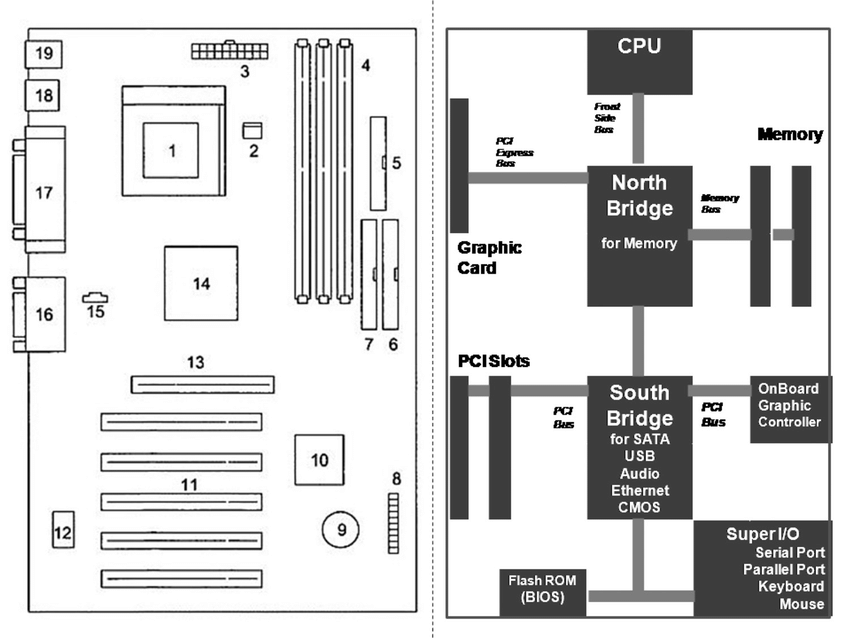
\includegraphics[width=1\linewidth,height=0.58\linewidth]{TVY-POS/Motherboard/MB.png}
Popis fyzického schéma:
\begin{enumerate}
  \item[1)] Patice CPU - Rozdíl mezi AMD (AM4, AM3) a Intel (12th gen LGA1700)
  \item[2)] CPU FAN Header - Pro chlazení CPU, jiné usazení chladiče pro AMD a Intel
  \item[3)] ATX napájení - Napájení základní desky a jejich komponent
  \item[4)] DDR sloty - Rozdíl mezi DDR3, DDR4, DDR5 (Umístění mezery)
  \item[8)] Porty pro case - HD Audio, USB, PWR, Reset, HDDLED, PWRLED
  \item[9)] RTC - Hodiny reálného času, baterie + kondenzátor, 32.768 kHz, 1.7 sekundy chyba denně
  \item[10)] Southbridge - Propojení NB a Serial \& Paralel port, PS2 klávesnice, myš
  \item[11)] PCI - Univerzální rozšiřující sloty. x4, x8, x16
  \item[12)] BIOS - Flash pamět se zaváděcím systémem
  \item[13)] PCI-E - Vysokorychlostní rožšiřující slot, v dnešní době hlavně pro grafické karty.
  \item[14)] Northbridge - Rozhraní pro propojení CPU s opereační pamětí a PCI-E
  \item[15)] FAN Header - Napájení a ovládání
  \item[] CPU napájení - Chybí na obrázku
\end{enumerate}